%% --------------------------------------------------------------
%%
%% R E S U L T S
%%
%% --------------------------------------------------------------

\section{Preliminary Results}
\subsection{Modelling sGRB afterglow (GRB170817A)}
\begin{frame}{}  %% ---------- Intro/motivation 
    \begin{tikzpicture}[overlay,remember picture]
        \uncover<1->{ % <-> |
            \node (t1) [anchor=center,scale=1,opacity=1] at ([shift={(-3.0cm,2.5cm)}]current page.center){
                \parbox{0.7\textwidth}{
                    \begin{itemize}
                        \item Gaussian jet $E(\theta) \propto e^{(\theta/\theta_c)^2}$
                        \item Off-axis $\theta_{\rm obs} > \theta_c$
                        \item Relativistic core, $\Gamma_c \sim 10^2$; low ISM density.
                    \end{itemize}
            }};
        }
        \uncover<1->{ % <-> |
            \node (img1) [anchor=center,scale=1,opacity=1] at ([shift={(1.cm,-1.35cm)}]current page.center){
                \parbox{1.0\textwidth}{
                    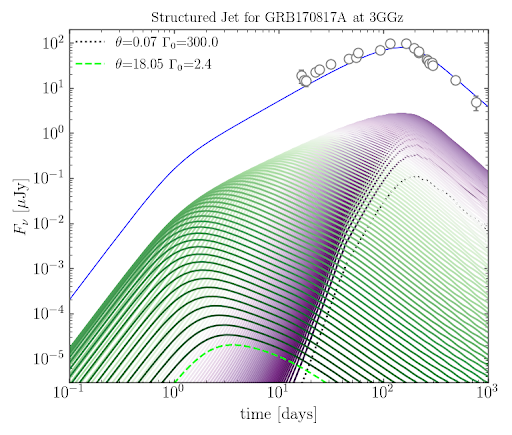
\includegraphics[height=6cm]{figures/grb170817fernandezPyBlastAfterglow.png}
            }};
        }
        \uncover<1->{ % <-> |
            \node (img1) [anchor=center,scale=1,opacity=1] at ([shift={(9.0cm,-0.5cm)}]current page.center){
                \parbox{1.0\textwidth}{
                    Flux centroid motion, $4.5\,$GGz; \\
                    Color is $I/I_{\rm max}$ %is shown with $I=0.01I_{\rm max}$ cut
                    
                    \movie[width=0.8\textwidth]{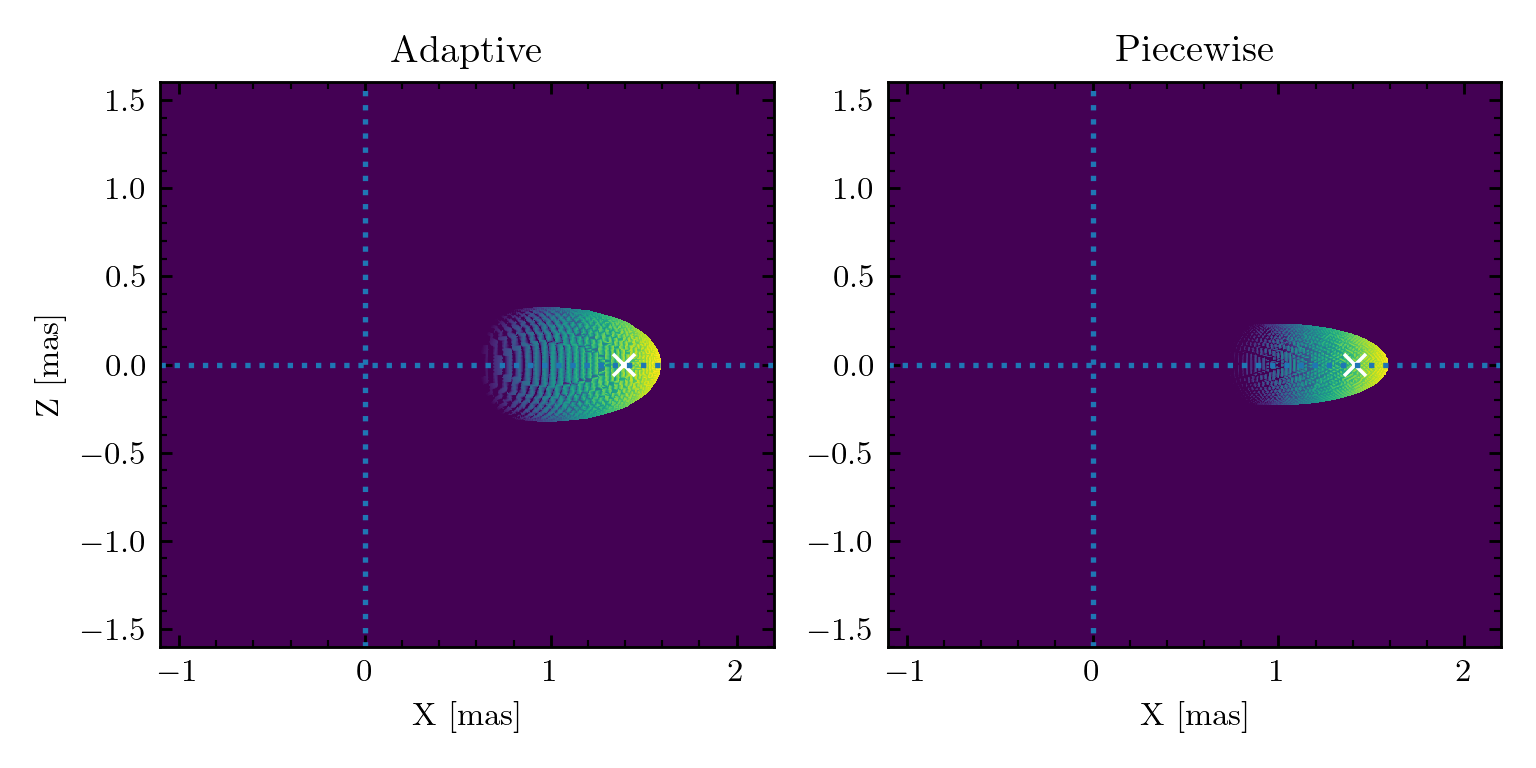
\includegraphics[width=0.8\textwidth]{figures/200.png}}{figures/out2.mp4}
            }};
        }
    \end{tikzpicture}
\end{frame}


% =============================================================================================

\subsection{Kilonova afterglow for NR ejecta profiles}
\begin{frame}{}  %% ---------- Intro/motivation 
    \begin{tikzpicture}[overlay,remember picture]
        \uncover<1->{ % <-> |
            \node (t1) [anchor=center,scale=1,opacity=1] at ([shift={(-3.1cm,-0.5cm)}]current page.center){
                \parbox{0.65\textwidth}{
                    %                    \textbf{Main Features}:
                    \begin{itemize}
                        \item Set of NS BNS simulations targeted to \GW{}.
                        %
                        \item BNS model $(q,\tilde{\Lambda})$ $q=M_A/M_B$ is the mass ratio, $\tilde{\Lambda}$ tidal deformability parameter (Depends in EOS of NS)
                        %
                        \item Ejecta $M,\beta,E_k = f(q,\tilde{\Lambda})$
                        %
                    \end{itemize}
                    
                    \textbf{Assuming that GRB170817A change in afterglow is due to the emergence of a new component}: 
                    \begin{itemize}
                        \item New way to constrain binary parameters, EOS
                        %
                        \item Additional information on ISM
                        %
                        \item Information on shock physics
                        %
                    \end{itemize}
            }};
        }
        \uncover<1-1>{ % <-> |
            \node (img1) [anchor=center,scale=1,opacity=1] at ([shift={(5.0cm,1.8cm)}]current page.center){
                \parbox{0.5\textwidth}{
                    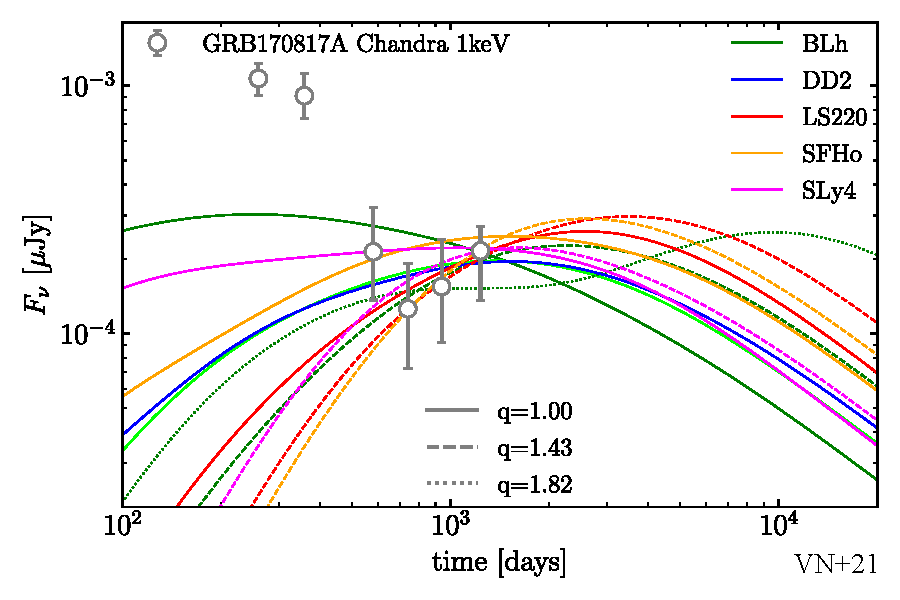
\includegraphics[height=3.8cm]{figures/best_xray_obs_representative_all_eos.pdf}
                    
                    %\small{\textbf{Artist depiction of ejecta$^\text{\citep{Ascenzi:2020xqi}}$}}
            }};
        }
        \uncover<1-1>{ % <-> |
            \node (img1) [anchor=center,scale=1,opacity=1] at ([shift={(5.2cm,-2.2cm)}]current page.center){
                \parbox{0.5\textwidth}{
                    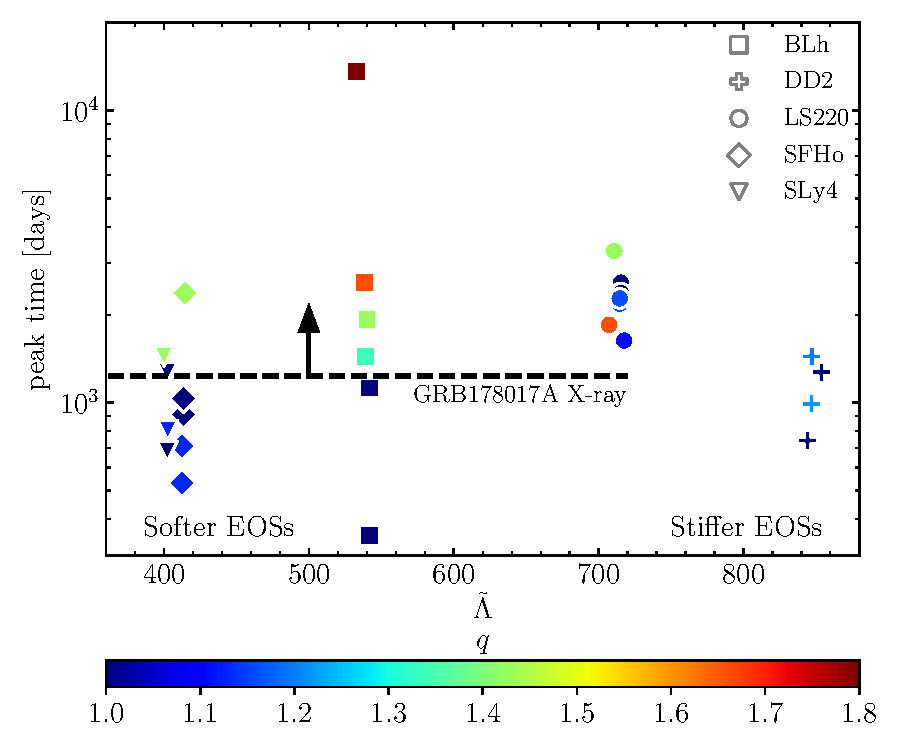
\includegraphics[height=4.2cm]{figures/scatter_lightcurve_tpeak_vs_lambda.pdf}
                    
                    %\small{\textbf{Artist depiction of ejecta$^\text{\citep{Ascenzi:2020xqi}}$}}
            }};
        }
    \end{tikzpicture}
\end{frame}

% =============================================================================================

\subsection{Thermal electrons in mildly relativistic shocks}
\begin{frame}{}  %% ---------- Intro/motivation 
    \begin{tikzpicture}[overlay,remember picture]
        \uncover<1->{ % <-> |
            \node (t1) [anchor=center,scale=1,opacity=1] at ([shift={(-3.0cm,2.2cm)}]current page.center){
                \parbox{0.5\textwidth}{
                    \begin{itemize}
                        \item ``Thermal spectrum'' (left)
                        \item ``Non-thermal spectrum'' (right)
                    \end{itemize}
                    $\beta_{\rm sh}=0.1$, $n_{\rm ISM}=10^4\,\ccm$, $t=200\,$d, $\delta=0.1$, $p=3$, $B=0.1\,$G, $\varepsilon_T=0.1$
            }};
        }
        \uncover<1->{ % <-> |
            \node (t1) [anchor=center,scale=1,opacity=1] at ([shift={(4.0cm,2.2cm)}]current page.center){
                \parbox{0.5\textwidth}{
                    \begin{eqnarray*}
                        \frac{\partial N}{\partial \gamma}\Big|_{\rm th} &= n_{e} \frac{ \gamma^2\sqrt{1-\gamma^{-2}} }{K_2(1/\Theta) \Theta} e^{-\gamma/\Theta}, \\
                        %                        \hspace{5mm}
                        \frac{\partial N}{\partial \gamma}\Big|_{\rm pl} &= n_e g(\Theta)\delta\frac{p-2}{3\Theta}\Big(\frac{\gamma}{3\Theta}\Big)^{-p}
                    \end{eqnarray*}
                    
                    
                    %                    Spectrum $3$ segments: 
                    %                    (i) $\nu < \nu_c$: low energy tail, $F_{\nu}\propto\nu^{1/3}$, 
                    %                    (ii) $\nu(\gamma) > \nu_c$ power law segment $F_{\nu}\propto\nu^{-1/2}$ 
                    %                    (iii) $\nu(\gamma)$and 
            }};
        }
        \uncover<1->{ % <-> |
            \node (img1) [anchor=center,scale=1,opacity=1] at ([shift={(2.cm,-1.5cm)}]current page.center){
                \parbox{1.0\textwidth}{
                    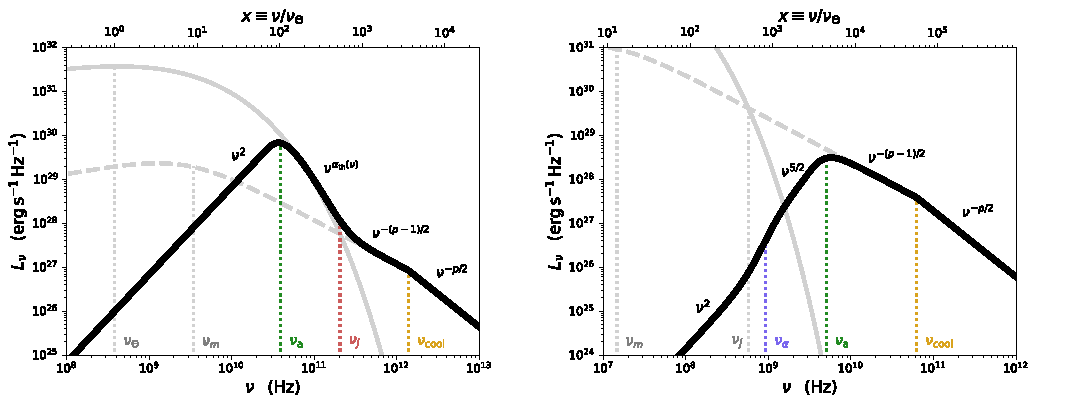
\includegraphics[height=5cm]{figures/Margalit21_thermalElectrons.pdf}
            }};
        }
    \end{tikzpicture}
\end{frame}
\begin{frame}{}  %% ---------- Intro/motivation 
    \begin{tikzpicture}[overlay,remember picture]
        \uncover<1->{ % <-> |
            \node (t1) [anchor=center,scale=1,opacity=1] at ([shift={(-5.0cm,1.2cm)}]current page.center){
                \parbox{0.4\textwidth}{
                    Comparison between two optically thin ight cruves:
                    \begin{itemize}
                        \item ``Thermal'' (blue)
                        \item ``Non-thermal'' (green)
                    \end{itemize}
                    Further investigations required! 
            }};
        }
        \uncover<1->{ % <-> |
            \node (img1) [anchor=center,scale=1,opacity=1] at ([shift={(6.cm,0.0cm)}]current page.center){
                \parbox{1.0\textwidth}{
                    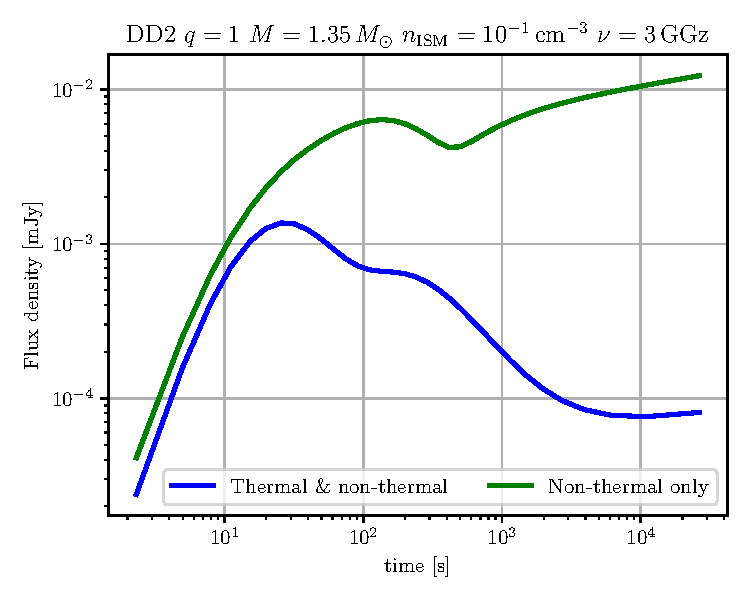
\includegraphics[height=7cm]{figures/test_thermal_electrons.pdf}
            }};
        }
    \end{tikzpicture}
\end{frame}

% =============================================================================================

\subsection{Extracting kilonova ejecta profile}
\begin{frame}{}  %% ---------- Intro/motivation 
    \begin{tikzpicture}[overlay,remember picture]
        \uncover<1->{ % <-> |
            \node (t1) [anchor=center,scale=1,opacity=1] at ([shift={(-3.0cm,2.5cm)}]current page.center){
                \parbox{0.7\textwidth}{
                    \begin{itemize}
                        \item $E_{\rm k} = f(\theta,\beta)$
                        \item $E_{\rm k;max}$ at $\theta\rightarrow0$ and $\beta\rightarrow0.2$.
                        \item $\log_{10}(E_k)=b_0 + (b_1 \theta) + (b_2 \beta) + (b_3 \theta^2) + (b_4 \theta \beta) + (b_5 \beta^{1/4})$
                    \end{itemize}
            }};
        }
        \uncover<1->{ % <-> |
            \node (img1) [anchor=center,scale=1,opacity=1] at ([shift={(2.2cm,-1.35cm)}]current page.center){
                \parbox{1.0\textwidth}{
                    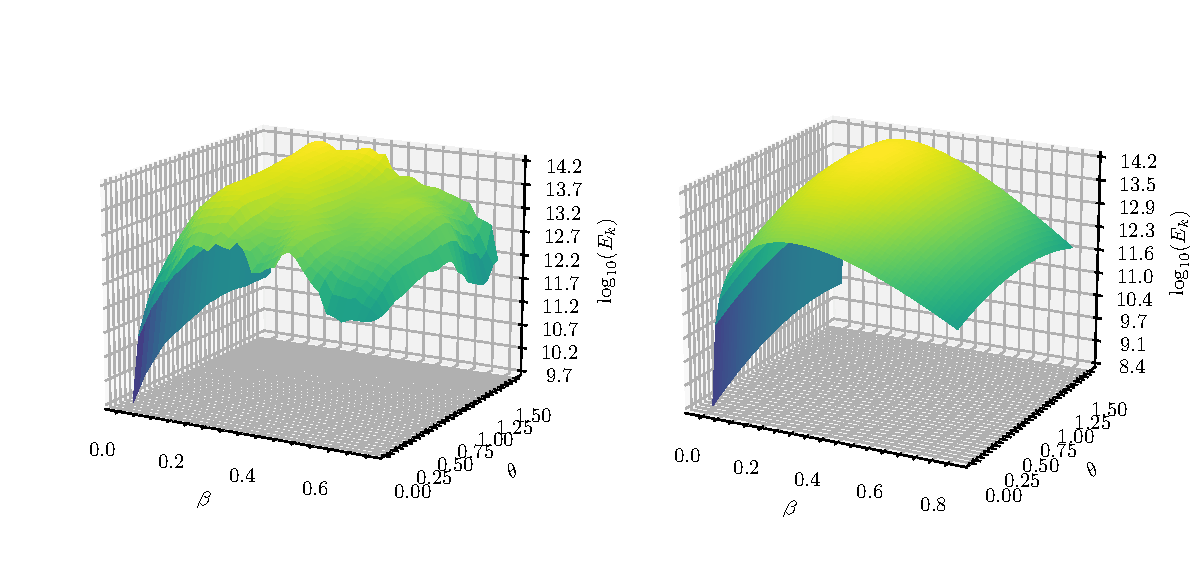
\includegraphics[height=6cm]{figures/fit_2d_ejecta.pdf}
            }};
        }
        \uncover<1->{ % <-> |
            \node (img1) [anchor=center,scale=1,opacity=1] at ([shift={(9cm,2cm)}]current page.center){
                \parbox{1.0\textwidth}{
                    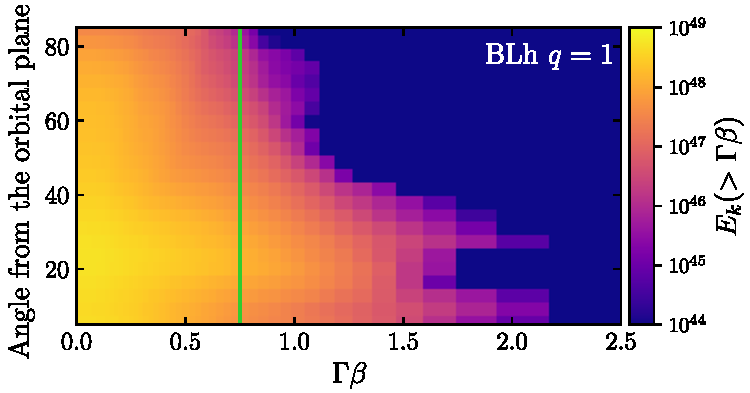
\includegraphics[height=3cm]{figures/kinetic_energy_struct_models_bottom_only.pdf}
            }};
        }
    \end{tikzpicture}
\end{frame}